% caffeine_dag.tex -- Knowledge-integration causal diagram
% (Pearl semi-Markovian / ADMG).
%   Revision 3: coupling reframed from mediator to observed indicator of a
%               latent shared knowledge base.
%   Revision 4 (2 Sept 2026): added the direct venue path V -> C, which both
%               statistical models already carried as a covariate on descent.
%
% Build:  xelatex caffeine_dag.tex  ->  caffeine_dag.pdf   (no shell-escape).
%
% PROVENANCE. The node and edge coordinates below were generated from REVISION 3
% of caffeine_dag.gv via
%   dot2tex --texmode=raw --format=tikz caffeine_dag.gv
% and then finished by hand: double-oval indicators, bow arc, notation key. The
% revision-4 edge V -> C is likewise hand-placed (marked in the body below).
%
% Re-running dot2tex on the current .gv will produce a DIFFERENT LAYOUT and will
% discard all of the hand finishing. This file, not the .gv, is what reproduces
% the figure as printed in caffeine_model_spec_outline.tex.
% Edit caffeine_dag.gv for STRUCTURE; this file for STYLING and LAYOUT.
%
% caffeine_dag_body.tex is this file's tikzpicture with the notation key removed,
% for inlining into the outline; keep the two in step.
\documentclass[11pt,border=10pt]{standalone}
\usepackage[x11names, svgnames, rgb]{xcolor}
\definecolor{gray25}{gray}{0.25}\definecolor{gray45}{gray}{0.45}
\definecolor{gray55}{gray}{0.55}\definecolor{gray60}{gray}{0.60}
\definecolor{gray93}{gray}{0.93}\definecolor{gray98}{gray}{0.98}
\definecolor{zred}{rgb}{0.69,0.19,0.19}
\usepackage{tikz}
\usetikzlibrary{arrows,shapes}
\usepackage{amsmath}\usepackage{bm}
\usepackage{fontspec}
\IfFontExistsTF{Latin Modern Roman}{\setmainfont{Latin Modern Roman}}{}

\begin{document}
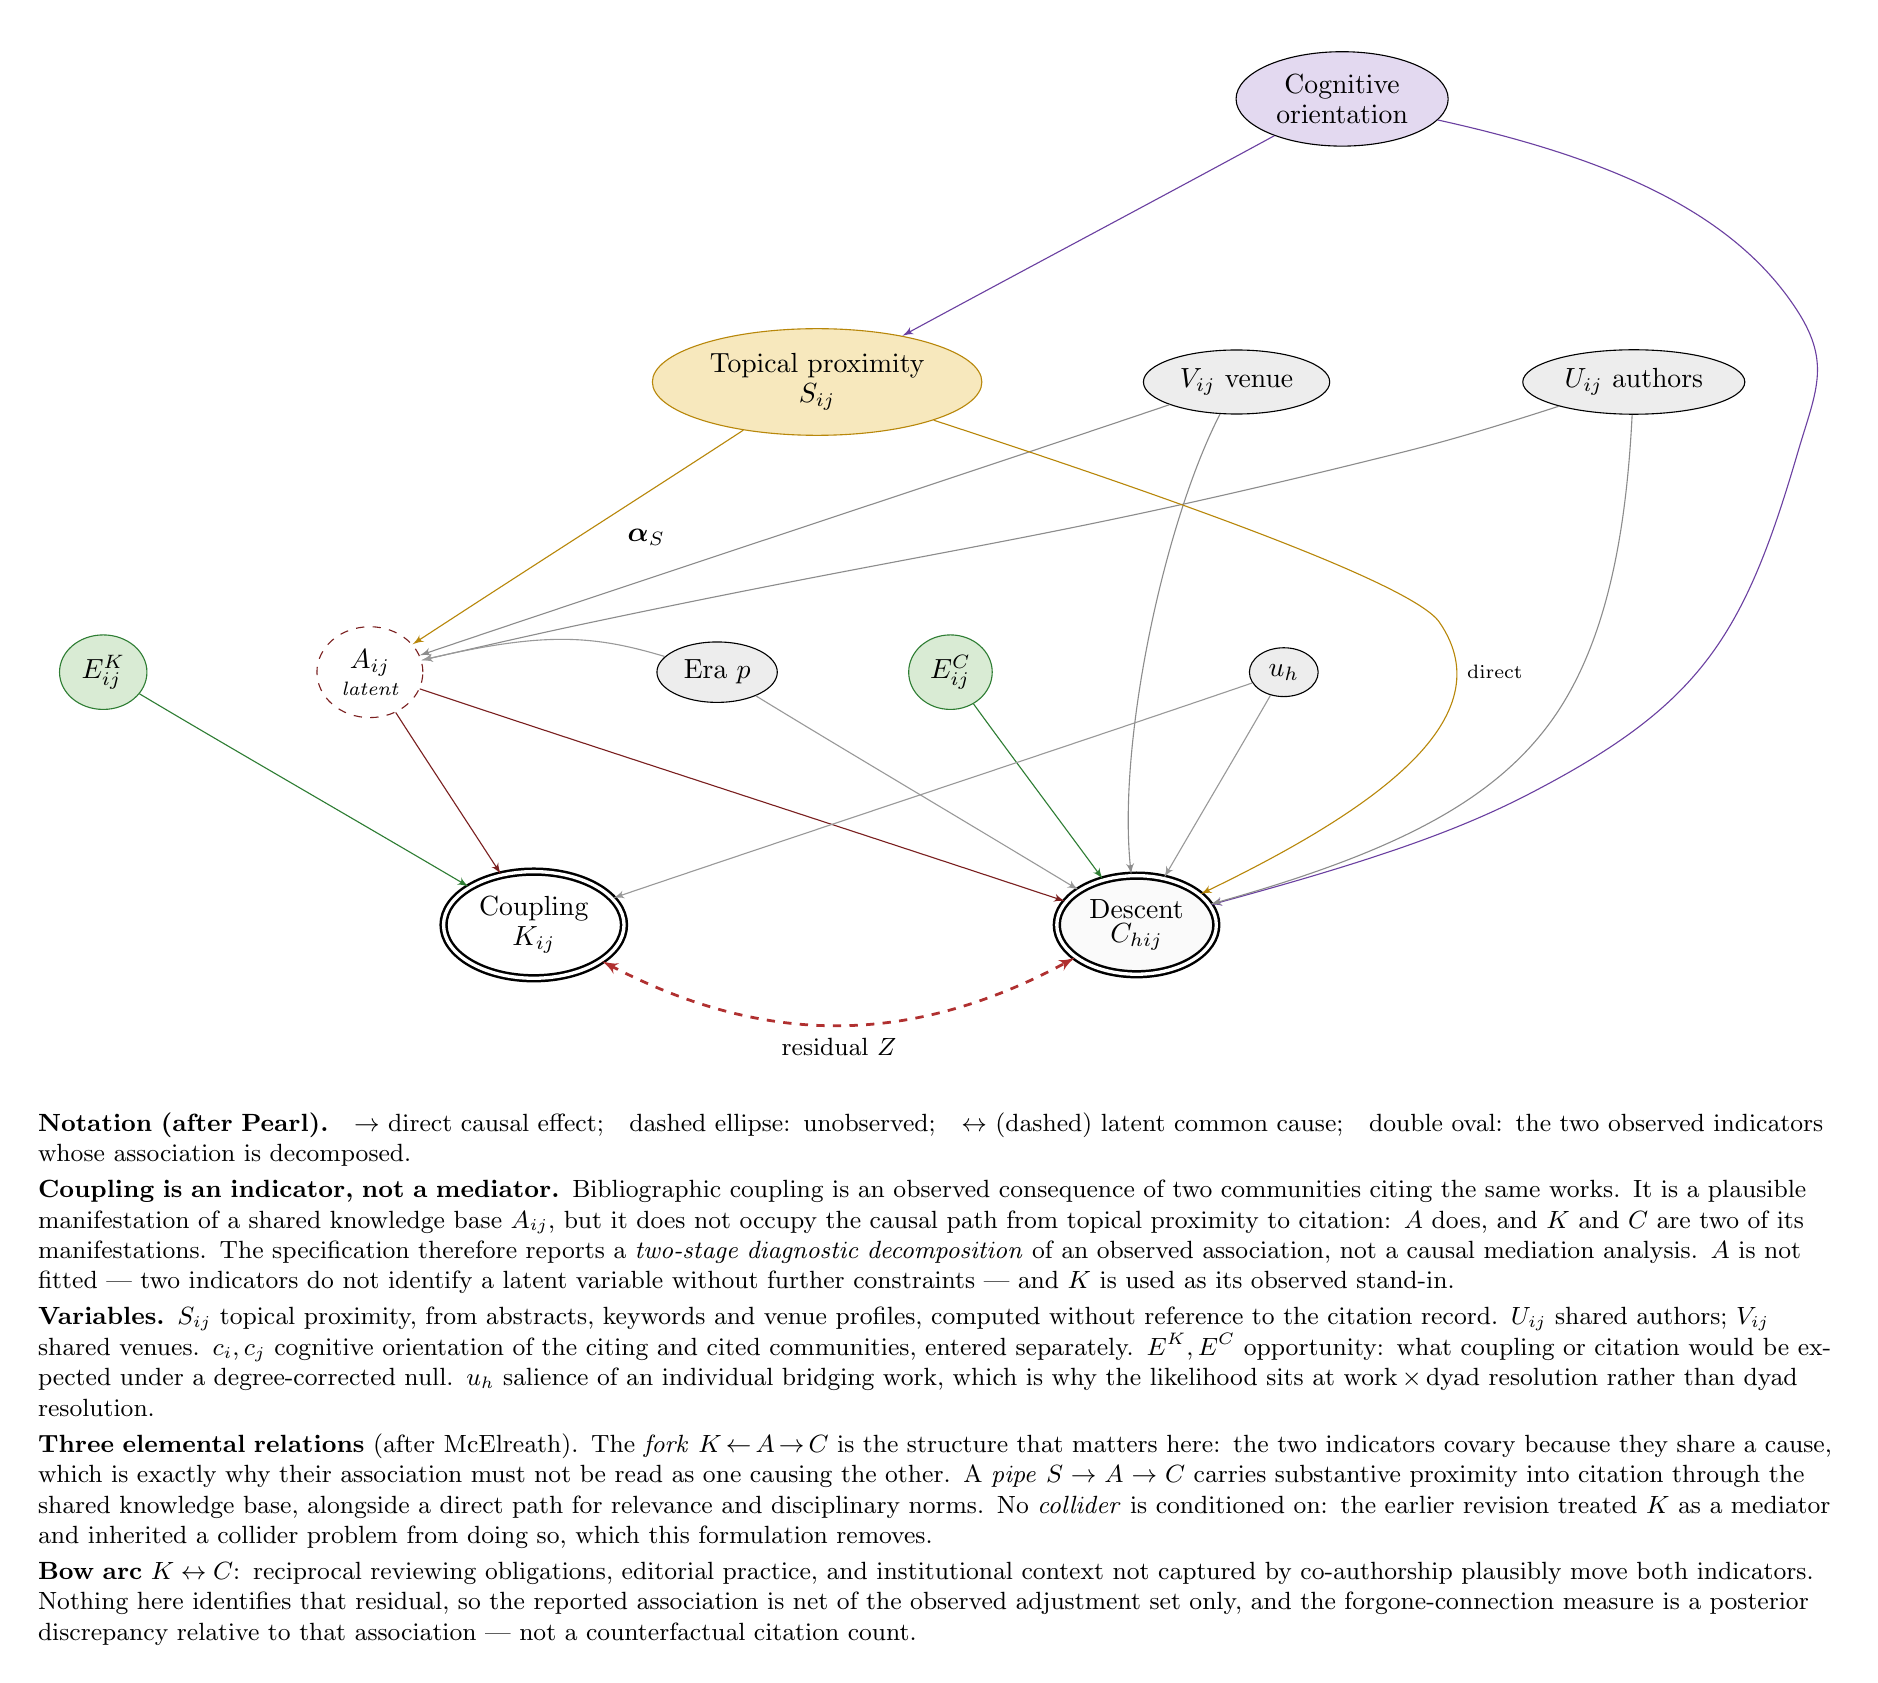
\begin{tikzpicture}[>=latex',line join=bevel,]
%%
\begin{scope}
  \pgfsetstrokecolor{black}
  \definecolor{strokecol}{rgb}{1.0,1.0,1.0}
  \pgfsetstrokecolor{strokecol}
  \definecolor{fillcol}{rgb}{1.0,1.0,1.0}
  \pgfsetfillcolor{fillcol}
  \fill [opacity=1] (0.0bp,0.0bp) -- (0.0bp,344.82bp) -- (644.32bp,344.82bp) -- (644.32bp,0.0bp) -- cycle;
  \draw [opacity=0.0] (0.0bp,0.0bp) -- (0.0bp,344.82bp) -- (644.32bp,344.82bp) -- (644.32bp,0.0bp) -- cycle;
\end{scope}
\begin{scope}
  \pgfsetstrokecolor{black}
  \definecolor{strokecol}{rgb}{1.0,1.0,1.0}
  \pgfsetstrokecolor{strokecol}
  \definecolor{fillcol}{rgb}{1.0,1.0,1.0}
  \pgfsetfillcolor{fillcol}
  \fill [opacity=1] (0.0bp,0.0bp) -- (0.0bp,344.82bp) -- (644.32bp,344.82bp) -- (644.32bp,0.0bp) -- cycle;
  \draw [opacity=0.0] (0.0bp,0.0bp) -- (0.0bp,344.82bp) -- (644.32bp,344.82bp) -- (644.32bp,0.0bp) -- cycle;
\end{scope}
\begin{scope}
  \pgfsetstrokecolor{black}
  \definecolor{strokecol}{rgb}{1.0,1.0,1.0}
  \pgfsetstrokecolor{strokecol}
  \definecolor{fillcol}{rgb}{1.0,1.0,1.0}
  \pgfsetfillcolor{fillcol}
  \fill [opacity=1] (0.0bp,0.0bp) -- (0.0bp,344.82bp) -- (644.32bp,344.82bp) -- (644.32bp,0.0bp) -- cycle;
  \draw [opacity=0.0] (0.0bp,0.0bp) -- (0.0bp,344.82bp) -- (644.32bp,344.82bp) -- (644.32bp,0.0bp) -- cycle;
\end{scope}
\begin{scope}
  \pgfsetstrokecolor{black}
  \definecolor{strokecol}{rgb}{1.0,1.0,1.0}
  \pgfsetstrokecolor{strokecol}
  \definecolor{fillcol}{rgb}{1.0,1.0,1.0}
  \pgfsetfillcolor{fillcol}
  \fill [opacity=1] (0.0bp,0.0bp) -- (0.0bp,344.82bp) -- (644.32bp,344.82bp) -- (644.32bp,0.0bp) -- cycle;
  \draw [opacity=0.0] (0.0bp,0.0bp) -- (0.0bp,344.82bp) -- (644.32bp,344.82bp) -- (644.32bp,0.0bp) -- cycle;
\end{scope}
\begin{scope}
  \pgfsetstrokecolor{black}
  \definecolor{strokecol}{rgb}{1.0,1.0,1.0}
  \pgfsetstrokecolor{strokecol}
  \definecolor{fillcol}{rgb}{1.0,1.0,1.0}
  \pgfsetfillcolor{fillcol}
  \fill [opacity=1] (0.0bp,0.0bp) -- (0.0bp,344.82bp) -- (644.32bp,344.82bp) -- (644.32bp,0.0bp) -- cycle;
  \draw [opacity=0.0] (0.0bp,0.0bp) -- (0.0bp,344.82bp) -- (644.32bp,344.82bp) -- (644.32bp,0.0bp) -- cycle;
\end{scope}
  \definecolor{fillcolor}{rgb}{0.89,0.85,0.94}
  \node (Cog) at (473.0bp,319.37bp) [draw,fill=fillcolor,ellipse] {\shortstack{Cognitive\\[-1pt]orientation}};
  \node (V) at (435.0bp,217.46bp) [draw,fill=gray93,ellipse] {$V_{ij}$ venue};
  \node (U) at (578.0bp,217.46bp) [draw,fill=gray93,ellipse] {$U_{ij}$ authors};
  \definecolor{strokecolor}{rgb}{0.72,0.53,0.04}
  \definecolor{fillcolor}{rgb}{0.97,0.91,0.74}
  \node (S) at (284.0bp,217.46bp) [draw=strokecolor,fill=fillcolor,ellipse] {\shortstack{Topical proximity\\[-1pt]$S_{ij}$}};
  \node (T) at (248.0bp,113.0bp) [draw,fill=gray93,ellipse] {Era $p$};
  \definecolor{strokecolor}{rgb}{0.48,0.12,0.12}
  \node (A) at (123.0bp,113.0bp) [draw=strokecolor,ellipse,dashed,fill=white] {\shortstack{$A_{ij}$\\[-1pt]{\scriptsize\itshape latent}}};
  \definecolor{strokecolor}{rgb}{0.18,0.49,0.2}
  \definecolor{fillcolor}{rgb}{0.85,0.92,0.83}
  \node (EK) at (27.0bp,113.0bp) [draw=strokecolor,fill=fillcolor,ellipse] {$E^{K}_{ij}$};
  \definecolor{strokecolor}{rgb}{0.18,0.49,0.2}
  \definecolor{fillcolor}{rgb}{0.85,0.92,0.83}
  \node (EC) at (332.0bp,113.0bp) [draw=strokecolor,fill=fillcolor,ellipse] {$E^{C}_{ij}$};
  \node (W) at (452.0bp,113.0bp) [draw,fill=gray93,ellipse] {$u_h$};
  \node (K) at (182.0bp,22.0bp) [draw,fill=white,ellipse,double,double distance=1.2pt,line width=0.9pt] {\shortstack{Coupling\\[-1pt]$K_{ij}$}};
  \node (C) at (399.0bp,22.0bp) [draw,fill=gray98,ellipse,double,double distance=1.2pt,line width=0.9pt] {\shortstack{Descent\\[-1pt]$C_{hij}$}};
  \definecolor{strokecolor}{rgb}{0.42,0.25,0.63}
  \draw [strokecolor,->] (Cog) ..controls (404.78bp,282.31bp) and (360.87bp,259.09bp)  .. (S);
  \definecolor{strokecolor}{rgb}{0.42,0.25,0.63}
  \draw [strokecolor,->] (Cog) ..controls (567.5bp,298.55bp) and (613.58bp,279.46bp)  .. (637.0bp,242.91bp) .. controls (649.21bp,223.86bp) and (643.35bp,213.72bp)  .. (637.0bp,192.0bp) .. controls (617.47bp,125.18bp) and (601.84bp,100.97bp)  .. (540.0bp,69.0bp) .. controls (513.73bp,55.422bp) and (482.66bp,44.769bp)  .. (C);
  \draw [gray55,->] (V) ..controls (337.04bp,184.29bp) and (226.56bp,148.01bp)  .. (A);
  % hand-placed: V -> C, direct venue path (see header note, revision 4)
  \draw [gray55,->] (V) ..controls (409.0bp,167.0bp) and (392.0bp,88.0bp)  .. (C);
  \draw [gray55,->] (U) ..controls (524.13bp,200.04bp) and (508.44bp,195.61bp)  .. (494.0bp,192.0bp) .. controls (365.8bp,159.95bp) and (332.3bp,158.29bp)  .. (203.0bp,131.0bp) .. controls (192.58bp,128.8bp) and (181.39bp,126.43bp)  .. (A);
  \draw [gray55,->] (U) ..controls (575.38bp,165.54bp) and (568.97bp,123.8bp)  .. (548.0bp,95.0bp) .. controls (526.39bp,65.322bp) and (489.23bp,47.332bp)  .. (C);
  \draw [gray60,->] (T) ..controls (202.97bp,126.48bp) and (185.66bp,127.54bp)  .. (A);
  \draw [gray60,->] (T) ..controls (292.89bp,85.542bp) and (331.36bp,62.865bp)  .. (C);
  \definecolor{strokecolor}{rgb}{0.72,0.53,0.04}
  \draw [strokecolor,->] (S) ..controls (224.33bp,178.49bp) and (183.06bp,152.22bp)  .. (A);
  \definecolor{strokecol}{rgb}{0.0,0.0,0.0}
  \pgfsetstrokecolor{strokecol}
  \draw (222.5bp,161.5bp) node {$\bm{\alpha}_S$};
  \definecolor{strokecolor}{rgb}{0.72,0.53,0.04}
  \draw [strokecolor,->] (S) ..controls (390.95bp,182.41bp) and (497.38bp,146.43bp)  .. (508.0bp,131.0bp) .. controls (531.78bp,96.472bp) and (485.13bp,63.579bp)  .. (C);
  \draw (528.0bp,113.0bp) node {{\scriptsize direct}};
  \definecolor{strokecolor}{rgb}{0.48,0.12,0.12}
  \draw [strokecolor,->] (A) ..controls (142.17bp,83.084bp) and (153.3bp,66.291bp)  .. (K);
  \definecolor{strokecolor}{rgb}{0.48,0.12,0.12}
  \draw [strokecolor,->] (A) ..controls (203.5bp,86.043bp) and (290.35bp,58.036bp)  .. (C);
  \definecolor{strokecolor}{rgb}{0.18,0.49,0.2}
  \draw [strokecolor,->] (EK) ..controls (70.909bp,86.788bp) and (111.69bp,63.372bp)  .. (K);
  \definecolor{strokecolor}{rgb}{0.18,0.49,0.2}
  \draw [strokecolor,->] (EC) ..controls (352.95bp,84.174bp) and (366.18bp,66.596bp)  .. (C);
  \draw [gray60,->] (W) ..controls (372.93bp,85.936bp) and (289.29bp,58.367bp)  .. (K);
  \draw [gray60,->] (W) ..controls (434.9bp,83.281bp) and (425.1bp,66.834bp)  .. (C);
%
%
  % --- hand-drawn bow arc: residual common causes beyond A and U ---
  \draw[<->,dashed,zred,line width=1.0pt] (K) to[bend right=28]
       node[pos=0.5,below=1pt,text=black,font=\small]
       {residual $Z$} (C);
  \pgfsetstrokecolor{black}
  \node[anchor=north west, align=left, text width=649bp, font=\small, text=black]
       at (0bp,-42bp) {%
    \textbf{Notation (after Pearl).}\quad $\rightarrow$ direct causal effect;\quad
    dashed ellipse: unobserved;\quad $\leftrightarrow$ (dashed) latent common cause;\quad
    double oval: the two observed indicators whose association is decomposed.\\[2pt]
    \textbf{Coupling is an indicator, not a mediator.} Bibliographic coupling is an
    observed consequence of two communities citing the same works. It is a plausible
    manifestation of a shared knowledge base $A_{ij}$, but it does not occupy the causal
    path from topical proximity to citation: $A$ does, and $K$ and $C$ are two of its
    manifestations. The specification therefore reports a \emph{two-stage diagnostic
    decomposition} of an observed association, not a causal mediation analysis. $A$ is
    not fitted --- two indicators do not identify a latent variable without further
    constraints --- and $K$ is used as its observed stand-in.\\[2pt]
    \textbf{Variables.} $S_{ij}$ topical proximity, from abstracts, keywords and venue
    profiles, computed without reference to the citation record. $U_{ij}$ shared
    authors; $V_{ij}$ shared venues. $c_i,c_j$ cognitive orientation of the citing and
    cited communities, entered separately. $E^{K},E^{C}$ opportunity: what coupling or
    citation would be expected under a degree-corrected null. $u_h$ salience of an
    individual bridging work, which is why the likelihood sits at work\,$\times$\,dyad
    resolution rather than dyad resolution.\\[2pt]
    \textbf{Three elemental relations} (after McElreath). The \emph{fork}
    $K\!\leftarrow\!A\!\rightarrow\!C$ is the structure that matters here: the two
    indicators covary because they share a cause, which is exactly why their association
    must not be read as one causing the other. A \emph{pipe}
    $S\!\rightarrow\!A\!\rightarrow\!C$ carries substantive proximity into citation
    through the shared knowledge base, alongside a direct path for relevance and
    disciplinary norms. No \emph{collider} is conditioned on: the earlier revision
    treated $K$ as a mediator and inherited a collider problem from doing so, which this
    formulation removes.\\[2pt]
    \textbf{Bow arc} $K\!\leftrightarrow\!C$: reciprocal reviewing obligations, editorial
    practice, and institutional context not captured by co-authorship plausibly move both
    indicators. Nothing here identifies that residual, so the reported association is net
    of the observed adjustment set only, and the forgone-connection measure is a posterior
    discrepancy relative to that association --- not a counterfactual citation count.};
\end{tikzpicture}
\end{document}
